% asset_id: FA22LinearCombinationsOfIndependentVariablesTikZ-001
% unit_code: FA22
% topic_code: FA22-LINCOMB
% topic_id: FA22LinearCombinationsOfIndependentVariables
% source: Phase 1 visual placeholder register
% purpose: Adding and subtracting random variables
\documentclass[tikz,border=10pt]{standalone}
\usepackage{amsmath}
\usepackage{tikz}
\begin{document}
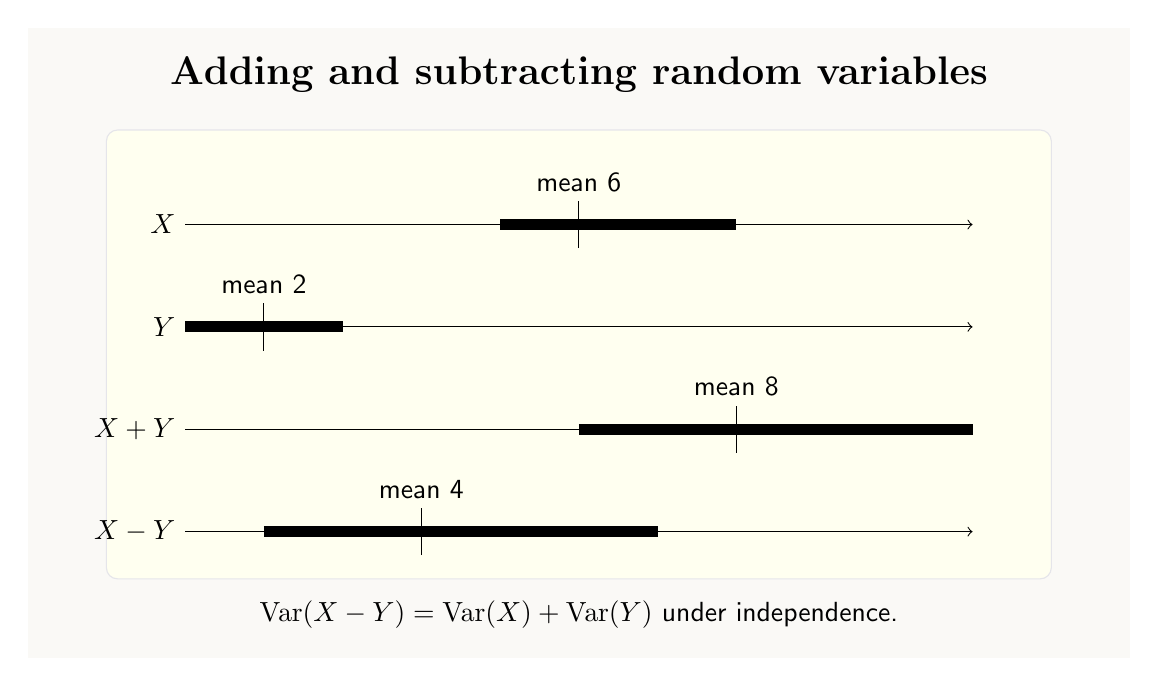
\begin{tikzpicture}[font=\sffamily]
\fill[fill={rgb,255:red,250;green,249;blue,246}] (-1,-1) rectangle (13,7);
\node[font=\bfseries\Large] at (6,6.4) {Adding and subtracting random variables};
\draw[rounded corners, fill={rgb,255:red,255;green,255;blue,240}, draw={rgb,255:red,229;green,229;blue,234}] (0,0) rectangle (12,5.7);


\draw[->] (1,4.5)--(11,4.5); \node[left] at (1,4.5) {$X$};
\draw[line width=4pt] (5,4.5)--(8,4.5); \draw (6,4.2)--(6,4.8); \node[above] at (6,4.8) {mean 6};
\draw[->] (1,3.2)--(11,3.2); \node[left] at (1,3.2) {$Y$};
\draw[line width=4pt] (1,3.2)--(3,3.2); \draw (2,2.9)--(2,3.5); \node[above] at (2,3.5) {mean 2};
\draw[->] (1,1.9)--(11,1.9); \node[left] at (1,1.9) {$X+Y$};
\draw[line width=4pt] (6,1.9)--(11,1.9); \draw (8,1.6)--(8,2.2); \node[above] at (8,2.2) {mean 8};
\draw[->] (1,0.6)--(11,0.6); \node[left] at (1,0.6) {$X-Y$};
\draw[line width=4pt] (2,0.6)--(7,0.6); \draw (4,0.3)--(4,0.9); \node[above] at (4,0.9) {mean 4};
\node at (6,-0.45) {$\operatorname{Var}(X-Y)=\operatorname{Var}(X)+\operatorname{Var}(Y)$ under independence.};

\end{tikzpicture}
\end{document}
